% This project is part of the Continuous-Function Estimator project
% Copyright 2019 the authors.

% to-do
% -----

% style notes
% -----------
% - line break at sentence breaks

%\documentclass[twocolumn]{aastex62}
%\documentclass[12 pt]{article}
\documentclass[modern]{aastex62}

\usepackage[sort&compress]{natbib}
\usepackage{graphicx}
\graphicspath{ {./images/} }
\usepackage{xspace}
\usepackage{xcolor}


% aastex parameters
%%\hypersetup{linkcolor=red,citecolor=green,filecolor=cyan,urlcolor=magenta}
\received{XXX}
%\revised{not yet}
\accepted{YYY}
%\submitjournal{ApJ}
\shorttitle{A Continuous Correlation Function Estimator}
\shortauthors{Storey-Fisher and Hogg}

% language
\newcommand{\cf}{2pcf\xspace} %2pF? 2PCF? %TODO: fix spacing after
% to capitalize or not to capitalize? leaning no
\newcommand{\Est}{The Continuous-Function Estimator\xspace}
\newcommand{\est}{the Continuous-Function Estimator\xspace}
\newcommand{\LS}{LS\xspace}
\newcommand{\foreign}[1]{\textsl{#1}}
\newcommand{\etc}{\foreign{etc}}
% math
\newcommand{\inv}{^{-1}}
\newcommand{\T}{^{\mathsf{T}}}
\newcommand{\hmpc}{$h^{-1}$Mpc}
% comments
\newcommand{\KSF}[1]{\textcolor{teal}{KSF says: #1}}
\newcommand{\hogg}[1]{\textcolor{red}{Hogg says: #1}}
%\newcommand{\KSF}[1]{\textcolor{teal}{}}

% margins
%\addtolength{\topmargin}{-0.75in}
%\addtolength{\textheight}{1.50in}

% affiliations
\newcommand{\ccpp}{\affiliation{%
    Center for Cosmology and Particle Physics,
    Department of Physics,
    New York University}}
\newcommand{\flatiron}{\affiliation{%
    Flatiron Institute, Simons Foundation}}
\newcommand{\cds}{\affiliation{%
    Center for Data Science,
    New York University}}
\newcommand{\mpia}{\affiliation{%
    Max-Planck-Institut f\"{u}r Astronomie, Heidelberg}}


\begin{document}\sloppy\sloppypar\raggedbottom\frenchspacing

\title{\textbf{Two-point statistics without bins: A continuous-function generalization of the correlation function estimator for large-scale structure}}
%Two-point statistics without bins: A correlation function estimator for large-scale structure in a continuous-function basis
%Two-point statistics without bins: The correlation function estimator for large-scale structure generalized to a continuous-function basis
%\title{\textbf{A Continuous-Function Estimator of the Correlation Function for Large-Scale Structure}}
%\title{\textbf{A Continuous Correlation Function Estimator for Large-Scale Structure}}
%\title{\textbf{A Continuous-Function Correlation Function Estimator for Large-Scale Structure}}
%\title{\textbf{Projecting the Correlation Function onto Continuous Functions for Large-Scale Structure Surveys}
%\title{\textbf{A Continuous Representation of the Correlation Function Estimator for Large-Scale Structure}}
%\title{\textbf{Correlation Function Estimation with Continuous Functions for Large-Scale Structure}}
%\title{\textbf{Estimating the Two-Point Correlation Function with Continuous Functions}}
%\title{\textbf{Projecting Two-Point Correlations onto General Basis Functions: A New Estimator For Large-Scale Structure}}
%\title{\textbf{A Correlation Function Estimator with General Basis Functions for Large-Scale Structure}}
%\title{\textbf{A Generalized Correlation Function Estimator For Large-Scale Structure}}
%\title{\textbf{No More Bins:\\ A Vectorized Correlation Function Estimator For Large-Scale Structure}}
%\title{A Generalized Correlation Function Estimator for Galaxy Surveys}

%Generalized Estimator?
%Projected Estimator?
%Continuous Estimator?
%Continuous-Function Estimator?
%Linear-Regression Estimator?
%Vectorized estimator?

\author[0000-0001-8764-7103]{Kate Storey-Fisher}
\ccpp

\author[0000-0003-2866-9403]{David W. Hogg}
\ccpp
\cds
\mpia
\flatiron

\begin{abstract}\noindent
% Context / Aims
The two-point correlation function (\cf) is the most important statistic in structure formation, used to measure the clustering of density field tracers (e.g. galaxies).
Current estimators of the 2pcf, including the standard Landy-Szalay (\LS) estimator, evaluate the \cf in hard-edged bins of separation between objects, which is inappropriate for the science context and results in a loss of information and a poor trade-off between bias and variance.
%Methods
We present a new estimator for the \cf, \emph{\est}, which generalizes \LS to a continuous representation and obviates binning in separation or any other pair property. 
Our estimator replaces the binned pair counts with a linear superposition of basis functions; it outputs the best-fit linear combination of basis functions to describe the \cf. 
It is closely related to the estimator used in linear least-squares fitting. 
The choice of basis can take into account the expected form of the \cf, as well as its dependence on properties other than separation.
%Results
We show that \est can estimate the clustering of artificial data in representations that provide more accuracy with fewer basis functions than \LS.
\Est achieves lower bias and lower variance than \LS. 
We also demonstrate that the estimator can be used to directly estimate the Baryon Acoustic Oscillation scale.
Critically, these will permit reductions in the number of mock catalogs required for covariance estimation, currently the limiting step in \cf measurements.
We discuss applications and limitations of \est for present and future studies of large-scale structure, including determining the dependence of clustering on galaxy properties and potentially unifying real-space and Fourier-space approaches to clustering measurements.

\end{abstract}

%TODO: should have 6 keywords 
%via Unified Astronomy Thesauras (UAT), http://astrothesaurus.org/concept-select/
\keywords{Astrostatistics techniques (1886), Baryon acoustic oscillations (138), Cosmology (343), Two-point correlation function (1951), Large-scale structure of the universe (902), Redshift surveys (1378)}

\section{Introduction}

The large-scale structure (LSS) of the Universe is critical to our understanding of fundamental cosmology. 
It encodes information about the physics of the early Universe and the subsequent expansion history.
In particular, LSS measures the Baryon Acoustic Oscillation (BAO) scale, which results from density fluctuations in the baryon-photon fluid.
The distance traveled by these density waves before recombination imprints a feature on the statistical description of the LSS, which can be used to determine the characteristic BAO length scale \citep{EisensteinHu1998}.
The LSS also contains the signature of redshift-space distortions caused by the peculiar velocities of galaxies, which are used to measure the growth rate of structure \citep{Kaiser1987}.
Additionally, the LSS can be used to constrain galaxy formation in conjunction with models of galaxy bias (e.g. \citealt{Hamilton1988}). %?
With current observations, the LSS is well-described by a cold dark matter model with a cosmological constant, the standard $\Lambda$CDM model.
Upcoming galaxy surveys will observe larger volumes with improved measurements, allowing us to test $\Lambda$CDM to even higher precision.

% MOVE TO THESIS INTRO
% We characterize the LSS by using luminous sources to trace the underlying matter density field.
% These tracers are often to taken to be galaxies, but can also be galaxy clusters, quasars and other sources; in this paper we will consider our tracers to be galaxies.
% The clustering of these objects is measured with two-point statistics, namely the power spectrum $P(k)$ and the two-point correlation function (\cf).
% These characterize the clustering in Fourier space and real space, respectively, with the \cf defined as the Fourier Transform of the power spectrum: 
% \KSF{i'm not sure about my notation here with the vectors and d3k}
% \begin{equation}
% \xi(\mathbf{r}) = \frac{1}{(2\pi)^3} \int P(\mathbf{k}) e^{i\mathbf{k} \cdot \mathbf{r}} d^3\mathbf{k}.
% \end{equation}
% If we assume isotropy, we find that the spherically averaged correlation function is
% \begin{equation}
% \xi(r) = \frac{1}{2\pi^2} \int_0^{\infty} P(k) \frac{\mathrm{sin}(kr)}{kr} k^2 dk.
% \end{equation}
% In principle, the power spectrum and the two-point correlation function contain the same information.
% However, in practical applications the survey boundaries introduce nontrivial issues in computing these statistics, leading to diverging approaches to their computation with a significant difference in expense.
% The \cf requires more computational power and extra survey products, but it is an incredibly useful tool; for instance, it well-suited to the analysis of the BAO feature which manifests at a single scale in real space.

The most important statistic for characterizing the LSS is the two-point correlation function (\cf).
The \cf measures the excess frequency at which any two galaxies are separated by a given distance, compared to a uniform distribution; effectively, it characterizes the strength of clustering at a given spatial scale. 
In calculating the \cf, the nontrivial survey boundaries of the surveys prevent us from directly summing pair counts.
% hogg: is the below important here? 
% TODO: move to sec 2!! 
To account for the survey boundaries as well as regions corrupted by issues such as bright foreground stars, a set of random points are Poisson-distributed within the acceptable survey window. 
The pairwise correlations of these unclustered points are used to normalize out the survey window when estimating the \cf of the clustered data.

%TODO: discuss choice here
The \cf is traditionally estimated in bins of radial separation.
This binning introduces inherent limitations.
First, the choice of bins requires a trade-off between bias and variance: fewer bins may bias the result, while more bins increases the variance of measurement.
Finite-width bins also result in a loss of information about the property in which one is binning.
As we work towards extreme precision in large-scale structure, maximizing the information we extract with our analyses will become increasingly important.
Finally, the error on the covariance matrix scales with the number of bins; a larger number of bins reduces bias, but means we must estimate a very large covariance matrix to achieve the required precision.
This is currently the limiting step in LSS analyses, requiring many mock catalogs tailored to the survey, and covariance matrix computation will further limit cosmological constraints as survey size increases.

More generally, binning adds arbitrary boundaries between continuous data; results should not depend on bin choice, yet they sometimes do.
\cite{Lanzuisi2017} noted that the choice of binning axis impacts the detected correlation between the luminosity of active galactic nuclei and their host galaxies; \cite{Grimmett2020} devised a method to investigate this correlation in a continuous manner using a hierarchical Bayesian model, eliminating the need for binning.
\cite{Bailoni2016} explored the dependence of clustering analyses on the number of redshift bins, finding a non-negligible difference in cosmological parameter uncertainties.
The implications for BAO analyses were explored by \cite{Percival2014}, who found that there is an optimal bin width given the analysis method.
This balances the increasing statistical error with small bins and the offset in the derived BAO peak location with large bins; the effects are small but non-negligible.
It is clear that, when analyzing smooth quantities such as LSS statistics, binning is sinning.
% at end of this paragraph, situate ourselves within that literature 
% think about if this paragraph were included in a future paper or review; what would it say about mine?

Estimators of the \cf have been studied extensively (\citealt{PeeblesHauser1974}; \citealt{DavisPeebles1983}; \citealt{Hamilton1993}).
The current standard estimator was proposed by \cite{LandySzalay1993}, hereafter \LS. It is based on summing all data pairs $DD$ with a given separation and using data-random pairs $DR$ and random pairs $RR$ to correct for the survey boundary. The \LS estimator of the correlation function $\hat{\xi}_k$ for the $k^\mathrm{th}$ bin in separation $r$ is
\begin{equation}
\hat{\xi}_k = \frac{DD_k - 2DR_k + RR_k}{RR_k}.
\end{equation}
Compared with other estimators based on simple combinations of $DD$, $DR$ and $RR$, \LS has been shown to have the lowest bias and variance \citep{Kerscher2000}.
Estimators of the \cf must also take into account the imperfect nature of the survey, including systematic effects, the target completeness, and fiber collisions.
To account for these, each galaxy pair is sometimes assigned a weight, and pair counts are replaced by the sum of pair weights.

Variations on the random catalog pair count method have been proposed in recent years.
\cite{Demina2016} replaced the $DR$ and $RR$ terms with an integral over the probability map, reducing computation time and increasing precision.
An estimator proposed by \cite{VargasMagana2013} iterates over sets of mock catalogs to find an optimal linear combination of data and random pair counts, reducing the bias and variance.
An alternative estimator, the marked correlation function (e.g. \citealt{WhitePadmanabhan2009}), avoids the use of a random catalog altogether: it considers the ratio between the \cf and a weighted correlation function in which weights are assigned based on galaxy properties, such as the local density.
These estimators have all taken probabilistic approaches; others have taken a likelihood approach.
\cite{BaxterRozo2013} introduced a maximum likelihood estimator for the \cf, which achieves lower variance compared to the \LS estimator, enabling finer binning and requiring a smaller random catalog for the same precision.
% TODO: kernel methods to cite and destroy here?
% minimal in intro: after lit review ("variations" paragraph) - in some ways what we're doing bears some resemblance to mcf, because we're weighting the pairs by functions, and kernel estimates bc we're projecting the pairs onto basis functions; we will discuss below that our method is distinct from both of these approaches. think of this careful address as talking to referree or referree-like reader

These estimators present improvements to \LS, but they are still limited to estimates in separation bins.
Some require additional computational costs or layers of complexity, so the standard formulation of \LS continues to be the default estimator used in most analyses.

In this paper, we present a new estimator for the correlation function, \est, which generalizes the \LS estimator to produce a continuous estimation of the \cf. 
\Est projects the galaxy pairs onto a set of continuous basis functions and computes the best-fit linear combination of these functions.
The basis representation can depend on the pair separation as well as other desired properties, and can also utilize the known form of the \cf.
For top-hat basis functions, \est exactly reduces to the \LS estimator. 
This estimator removes the need for binning and allows for the \cf to be represented by fewer basis functions, requiring fewer mock catalogs to compute the covariance matrix.
It is particularly well-suited to the analysis of LSS features such as the BAO peak; we find that we can accurately locate the peak with fewer components.

%will obviously keep changing this as paper develops
This paper is organized as follows. 
In $\S$\ref{sec:motiv}, we motivate our estimator and explain its formulation.
%In Section \ref{sec:est}, we prove its correctness and describe our implementation, and demonstrate its application on a simulated data set. 
%Our results on the SDSS LRG sample are shown in Section \ref{sec:app}. 
We demonstrate its application on a simulated data set, including a toy BAO analysis, in $\S$\ref{sec:app}.
We discuss the implications and other possible applications in $\S$\ref{sec:discuss}. 

\section{Motivation and Formulation} 
\label{sec:motiv}

\subsection{Standard Clustering Estimation}

We assume we have a data catalog with $N_D$ objects and a random catalog with $N_R$ objects.
The pair counts for \LS and related estimators are then defined explicitly as
%TODO: fix spacing on sides of equal sign
\begin{eqnarray}\displaystyle
\label{eq:ls1}
DD_k &\equiv& \frac{2}{N_D(N_D-1)} \sum_{n n'} i(g_k < |x_n - x_{n'}| < h_k) \\ 
DR_k &\equiv& \frac{1}{N_D N_R} \sum_{n m} i(g_k < |x_n - x_m| < h_k) \\
\label{eq:ls3}
RR_k &\equiv& \frac{2}{N_R(N_R-1)} \sum_{m m'} i(g_k < |x_m - x_{m'}| < h_k),
\end{eqnarray}
where $DD_k$ is the count of data--data tracer pairs in bin $k$ (which has bin edges $g_k$ and $h_k$), $i()$ is an indicator function that returns $1$ if the the condition is true and otherwise returns $0$, $x$ is the tracer position, the $n$ and $n'$ indices index data positions, the $m$ and $m'$ indices index random catalog positions, $DR_k$ is the count of data--random pairs, and $RR_k$ is the count of random--random pairs.
The tracer position can be in real or redshift space, or broken down into the transverse and line-of-sight directions in the anisotropic correlation function; in this paper we consider the isotropic real-space \cf for simplicity, but the estimators detailed here apply equally well to these alternative configurations.
Our results here also apply in a straightforward way to the cross-correlation; for details see \S\ref{ref:beyondls}. 

The \LS estimator is known to be optimal (i.e. it is unbiased and has minimum variance) under a particular set of conditions: in the limit of unclustered data, for a data volume much larger than the scales of interest, and an infinitely large random catalog. 
In practice the latter two limits are sufficiently satisfied, but the data we are interested in are clustered.
\cite{VargasMagana2013} show that for clustered data, the \LS estimator has lower variance than other estimators, but does not reach the Poisson noise limit.
When applied to clustered data, \LS does show a bias on very large scales ($>$130 \hmpc), but the bias is significantly smaller than that of most other estimators (\citealt{Kerscher1999}, \citealt{VargasMagana2013}).
\LS is also less sensitive to the number of random points than other estimators \citep{Kerscher2000}.
While \LS has been sufficient for past analyses, its persisting bias and suboptimal variance under imperfect conditions mean that improvement is possible, and will be necessary for realistic large-scale structure measurements on modern datasets.

\subsection{Least Squares Fitting}

Estimating clustering is closely related to least-squares fitting.
We are essentially trying to find the best representation of spatial data in the space of two-point radial separation.
Recall that the linear least-squares fit to a set of data is
\begin{equation}
X = [A\T C\inv A]\inv [A\T C\inv Y]
\end{equation}
where $X$ is the vector of best-fit parameters, $A$ is a design matrix with zeroth and first order terms (and possibly higher order) functions of fitting features, $C$ is the covariance matrix, and $Y$ is a column vector of $y$ data to be fit.
The second bracketed term projects the data onto the features; the first bracketed term renormalizes this quantity. \KSF{renormalizes what??}
In the case of the \cf, the observed data is the pair counts at a given separation, and the weights are provided by the pair counts of the random catalog.
Indeed, this is reminiscent of the so-called natural estimator of the \cf, $\xi_k = DD_k/RR_k - 1$ (e.g. \citealt{Kerscher2000}).

From this connection, we can infer the form of the estimator.
\KSF{What else to say in this section?? How to expand on what's here?}

% TODO: fix this capitalization issue
\subsection{\Est}
\label{sec:est}

\KSF{Q about notation; I switched from the sub-k notation to vector notation, because these need to be vectors / tensors to then compute the amplitude. But this might be adding additional confusion. I could write DD, RR etc in k-notation, and then switch to vector notation for the amplitude and evaluation equations? Thoughts?}
Inspired by least-squares fitting, we generalize the \LS estimator defined above in Equations \ref{eq:ls1}-\ref{eq:ls3}.
We generalize the indicator function $i$ to any function $f$.
We further generalize the arguments of the function to any properties of the galaxies, rather than just their separation. 
Writing these now in vector notation, with $f$ returning a vector of length $K$ where $K$ is the number of ``basis functions'', we have
\KSF{I introduced this T notation to be the most general, as f can be a function of any galaxy properties, not just separation (which would be e.g. $r_{nm}$), but it's a bit clunky - especially when it comes to evaluating xi at the amplitudes. Thoughts?}
\KSF{we should double count so that we could be sure to be symmetric; change 2->1 and say that we explicitly double count here. tho in an implementation we might not, and then prefactor changes. also say that the notation, sum over n n', does not self add. if want to be explicit, use double sum. think i should do this... then need to do double sum for LS def. for my version, write it as parallel as possible as LS, and call out changes. RR and DR now vectors, QQ is tensor}
\KSF{vectors should be bolded; DD DR RR, f, ...}
\begin{eqnarray}\displaystyle
DD &\equiv& \frac{2}{N_D(N_D-1)} \sum_{n n'} f(T_n, T_{n'}) \\
DR &\equiv& \frac{1}{N_D N_R} \sum_{n m} f(T_n, T_{m}) \\
RR &\equiv& \frac{2}{N_R(N_R-1)} \sum_{m m'} f(T_m, T_{m'}) \\
QQ &\equiv& \frac{2}{N_R(N_R-1)} \sum_{m m'} f(T_m, T_{m'}) \cdot f\T(T_m, T_{m'}), \label{eq:qq_proj}
\end{eqnarray}
where $DD$, $DR$, and $RR$ are now $K$-vectors, $T$ refers to the data for the given tracer, and $QQ$ is a $K$-by-$K$ tensor defined as the outer product of basis function evaluations of the random--random pairs.
\KSF{what do we think about K-vector notation? K is number of basis functions / components, as stated above}

Then, we can compute the \cf as
\begin{eqnarray}\displaystyle
% here is where the T notation is weird - when you look at evaluation
a &\equiv& QQ\inv \cdot (DD + 2DR - RR) \\
\xi(T_l, T_{l'}) &\equiv& a\T \cdot f(T_l, T_{l'}) \label{eq:xi_proj}
\end{eqnarray}
where $T_l$ and $T_{l'}$ contain the data values at which to evaluate $\xi$, and $a$ is a $K$-vector of the ``amplitudes'' of the basis functions.

We call this generalized \cf estimator \est.
It replaces the binned pair counts of \LS with any set of basis functions. 
The linear superposition of these basis functions is the \cf.
\Est outputs the best-fit linear combination of basis functions to describe the \cf.
In this sense, it is related to the linear least-squares fitting described above.
With this formulation, we no longer need to first bin our data and then fit a function; rather, the estimator directly projects the data (the pair counts) onto the desired function.
This function can be nearly anything; the only limitation is it must be able to be written as a linear combination of basis functions.

\KSF{What do you think of the ordering of these paragraphs?}
We can recover the Landy-Szalay estimator with the proper choice of $f$ and $T$.
From our full galaxy pair data $T_n$ and $T_{n'}$, we can use only their separation,  $|x_n - x_n'|$.
We can then define a set of basis functions $f\T$ as,
\begin{equation}
f\T_k(T_n, T_{n'}) =  i(g_k < |x_n - x_{n'}| < h_k)
\end{equation}
where $k$ denotes a particular bin in separation.
This is the top-hat or rectangular function.
In this case the $DD$, $DR$ and $RR$ vectors simply become binned pair counts, with diagonal elementsm with $g_k$ and $h_k$ the bin edges as before.
The $QQ$ tensor becomes diagonal, with its diagonal elements equal to the $RR$ vector elements.
Then the evalution of the amplitudes and $\xi$ results in the equivalent of the \LS estimator--just displayed in a continuous form.

With this generalized two-point estimator, the basis functions $f$ need not have hard edges like the top-hat function.
They can instead be smooth functions of the pair separation, chosen to suit the science use case.
Further, the bases can make use of other information about the tracers, such as galaxy luminosity.
\KSF{should I note here that we don't explore this further in this paper?}
The estimator has the property that it is invariant under affine transformations; we show this in Appendix \ref{sec:affine}. \KSF{What more should I say about this? Why is it important? ``it is invariant under affine transformations, as it should be so that the result does not depend on e.g. the magnitude of the bases''?}

We can also write down the form of the estimator when we don't need to worry about the survey window; i.e. when we are working with a periodic box.
In this case, we can analytically compute the $RR$ term, as well as the $QQ$ term, and use the natural form of the \cf estimator.
The derivation and formulation of these terms are shown in Appendix \ref{sec:analytic}.

\KSF{Discuss the limit of infinitesimal bins? Do we know what this is?} \hogg{Yes, we should discuss this, and show how we are related to that.} \KSF{I'm not sure what to say about this.}

We implement this estimator based on the correlation function package \texttt{Corrfunc} by \cite{Sinha2019}.
\texttt{Corrfunc} is the state-of-the-art package for computing correlation functions and other clustering statistics; it is extremely fast and user-friendly, and is used in many published analyses.
It is also modular and open-source, making it a natural choice as a base for our implementation.
Our implementation of \est is also open-source and available at \texttt{github.com/kstoreyf/Corrfunc}.


\section{Experiments and Results}
\label{sec:app}

We demonstrate the application of \est on artifical data.
We generate lognormal mock catalogs \citep{ColesJones1991} using the \texttt{nbodykit} package \citep{Hand2018}.
We use an input power spectrum with the Planck cosmology \KSF{CITE}.
The true correlation function is then known: it is the Fourier transform of the input power spectrum, computed numerically.
Our test catalogs have size (750 \hmpc)$^3$ and a galaxy number density of $3 \times 10^{-4}$, to match that of the Brightest Cluster Galaxies \KSF{CITE}.
We construct 100 realizations of this box. 
We also generate a uniformly sampled random catalog with 10 times the number of galaxies as in the data catalogs.

\subsection{Demonstration using Spline Basis Functions}
\label{sec:spline}

\label{fig:spline}
\begin{figure}[ht]
\centering
    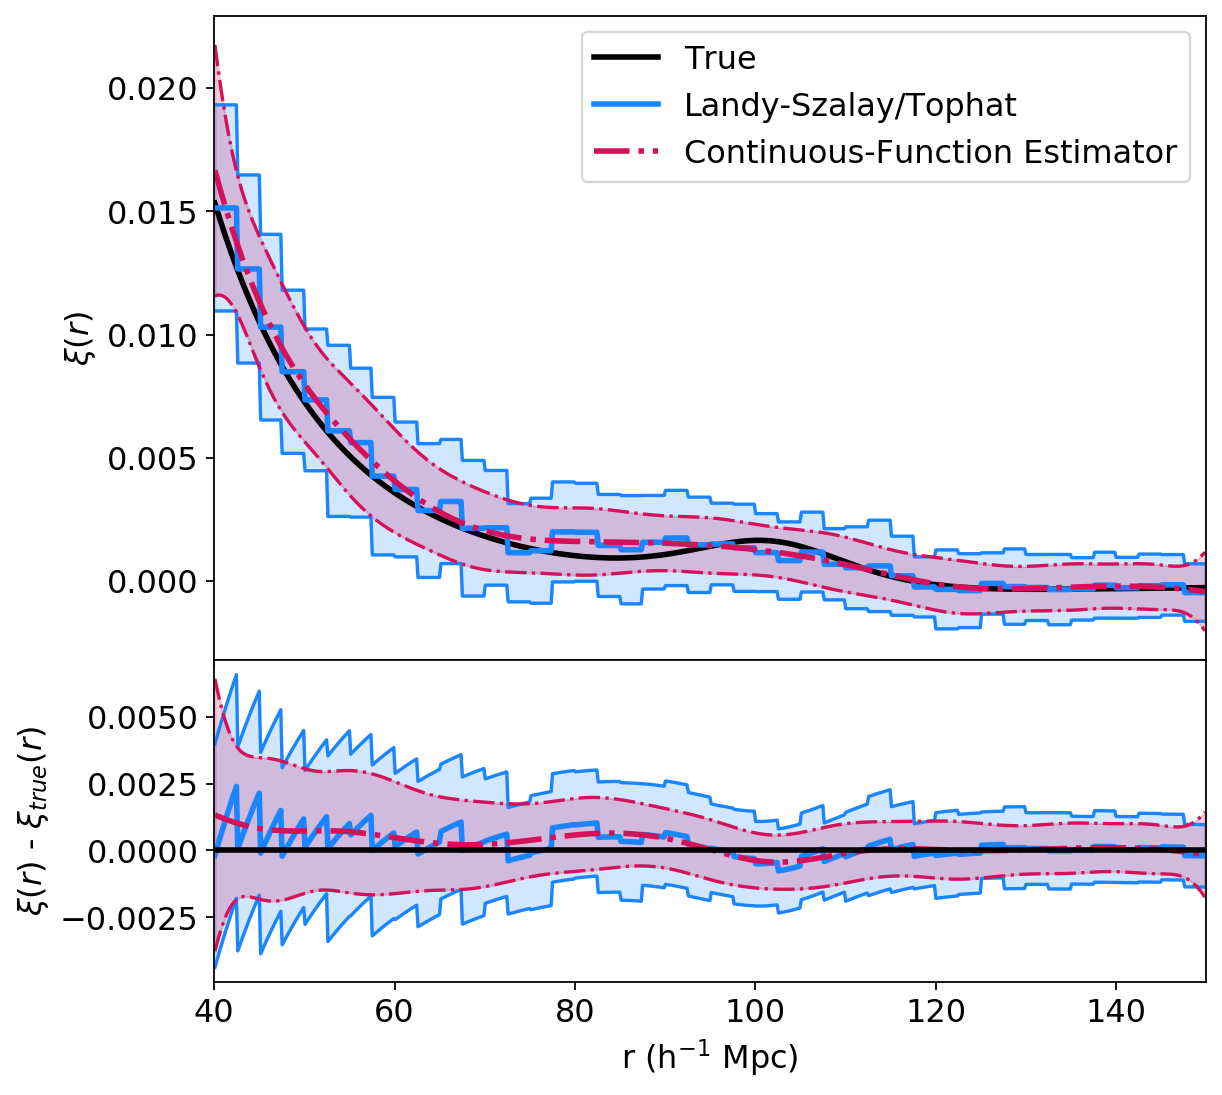
\includegraphics[width=0.8\textwidth]{tophat_cubic}
    \caption{A comparison between \est with a cubic spline basis function (red dotted) and the standard tophat estimator (blue solid). The shaded region is the 1$\sigma$ variation in the 100 mock catalogs. The cubic spline estimator has lower bias and lower variance with fewer bins. \KSF{quote rmse in caption? otherwise not clear from figure its less biased.} \hogg{yes} \KSF{does tophat need to be a different linestyle?}} \KSF{fix to dotted linestyle}

\end{figure}

\KSF{Should i have a figure showing the basis functions?} \hogg{yes}

A natural extension of tophat basis functions is the B-spline.
B-splines of order $n$ are piecewise polynomials of order $n-1$; they constitute the basis functions for spline interpolation \KSF{CITE}.
They have the nice property that the functions and their derivatives can be continuous, depending on the order.
Further, B-splines are well-localized, which provides a more direct comparison to the typical tophat basis (which is entirely localized).
For this demonstration we use fourth-order B-splines, which constitute the set of basis functions for a cubic spline, as they are the lowest-order spline to have a continuous first derivative.
We compare this standard estimator, reformulated as continuous functions using a tophat basis.
For the tophat basis we use 44 basis functions in the range $40 < r < 150$ \hmpc, each with a width of 2.5 \hmpc. 
For the cubic spline basis, we use the same $r$ range, but with only 11 basis functions, and knots chosen on a grid of 10 \hmpc.
\KSF{need to specify more about knots? is this accurate (not quite, the knots repeat values at the edge i think...) and should i mention control points?}

The results are shown in Figure~\ref{fig:spline}, compared to the true input \cf.
The spline basis results in a \cf estimate that has a root mean square error (RMSE) with respect to the truth of $4.38 \times 10^{-4}$, compared to $5.31 \times 10^{-4}$ for the tophat basis.
This holds true when we average over the bin \KSF{need to do weighted average based on which r-values contribute? supposed to hear from tinker}, as in standard practice, and then compute the RMSE.
The spline basis also results in lower variance across the 100 mocks, compared to the tophat basis.
Thus, \est allows for a more accurate and precise estimate of the \cf with fewer components.

We note that this is fundamentally different than a kernel-based estimator.
In a kernel formulation, each data point is smoothed by a particular kernel, smoothing out features in the resulting function.
With our estimator, the basis functions are fixed and the data is projected onto them.
This preserves the information in the data to the degree given by the chosen set of basis functions, which can in fact enhance features rather than smooth them.
\KSF{please add/correct here}

\subsection{BAO Scale Estimation Test}

Measurement of the BAO scale provides a good use case for our estimator.
The BAO feature is a peak in clustering on large scales, $\sim$150 Mpc, making it less sensitive to small-scale astrophysical effects.
It is one of the best tools for constraining cosmological models, in particular the distance-redshift relation \citep{Kazin2010, Anderson2012, Anderson2014, Alam2016}.

\KSF{what else do I need to cite for BAO?}

We base our BAO estimation on the method of the BOSS DR10 and 11 analysis \citep{Anderson2014}.
We measure the spherically averaged correlation function, $\xi(s)$, where $s$ is the separation between pairs.
In order to extract information about the baryon acoustic feature from galaxy clustering, we must choose a fiducial cosmological model to convert redshifts to distances.
If we choose an incorrect model, the scales in the power spectrum will be dilated, so the oscillation wavelength---and thus the BAO peak position---will be shifted.
We can model this shift as a scale dilation parameter, $\alpha$, which is a function of the relevant distance scales in the true and fiducial cosmologies:
\begin{equation}
\alpha = \Bigg( \frac{D_A(z)}{D_A^{\text{mod}}(z)} \Bigg)^{2/3} \Bigg( \frac{H^{\text{mod}}(z)}{H(z)} \Bigg)^{1/3} \Bigg( \frac{r_s^{\text{mod}}}{r_s} \Bigg),
\end{equation}
where $D_A$ is the angular diameter distance, $H$ is the Hubble constant, $r_s$ is the sound horizon scale at the drag epoch, and the superscript ``$\text{mod}$'' denotes the value for the fiducial model.
Qualitatively, if the fit prefers $\alpha>1$, this suggests the true position of the BAO peak is at a smaller scale than in the fiducial model, whereas if $\alpha<1$, the peak is at a larger scale.

% Using spherically averaged so don't need this!!
% The multipoles of the correlation function are given by
% \begin{equation}
% \xi_l(s) = \frac{1}{2} \int^{1}_{-1} \xi_l(s, \mu) L_l(\mu) d\mu
% \end{equation}
% where $L_l$ is the Legendre multipole of order $l$,  $s$ is the redshift-space separation between pairs, and $\mu = cos(\theta)$, $\theta$ is the angle between the separation vector $s$ and the line-of-sight direction (i.e. $\mu=1$ indicates a galaxy pair along the line of sight, $\mu$=0 indicates a pair with only transverse separation).

In standard practice, the fitting function used to determine the value of $\alpha$ is
\begin{equation}
\xi^{\text{fit}}(s) = B^2 \xi^{\text{mod}}(\alpha s) + \frac{a_1}{s^2} + \frac{a_2}{s} + a_3
\end{equation}
where $B$ is a constant that allows for a large-scale bias, and $a_1$, $a_2$, and $a_3$ are nuisance parameters to account for the broadband shape.
A $\chi^2$ fit is performed with five free parameters: $\alpha$, $B$, $a_1$, $a_2$, and $a_3$.
The resulting value for $\alpha$ is used to derive the actual values of the distance scales of interest.
Typically, density-field reconstruction is performed before applying the estimator to correct for nonlinear growth around the BAO scale \citep{Eisenstein2007}; for our toy example, we will omit this step.

The form of the standard fitting function is well-suited to our estimator, as it is a few-parameter model with a linear combination of terms.
To use our estimator to estimate $\alpha$, we take the numerical partial derivative of the model with respect to $\alpha$, using a change in $\alpha$ of size $d\alpha$.
Our fitting function is then
\begin{equation} \label{eq:baoiter_fit}
\xi^{fit}(s) = B^2 \xi^{mod}(s) + C d\alpha\frac{d\xi_{mod}(\alpha s)}{d\alpha} + \frac{a_1}{s^2} + \frac{a_2}{s} + a_3,
\end{equation}
where $C$ describes the contribution of $\alpha$.
We input these five terms (with arbitrary scaling) as the basis functions of our estimator.
The estimator outputs an amplitude vector $a$ as described in $\S$\ref{sec:est}, which give the contribution of each term---precisely the values of $B$, $C$, $a_1$, $a_2$, and $a_3$.
From the value of $C$, we can directly compute $\alpha$, as $\alpha_{\text{recovered}} =  \alpha + Cd\alpha$ (where $\alpha$ is our initial guess, typically starting with  $\alpha$=1). 
That is, a value of $C=0$ indicates that the model is the best fit to the data and no scale dilation is needed, while nonzero values give the magnitude and direction of the scale dilation parameter.

\label{fig:bao_bases}
\begin{figure}[ht]
\centering
    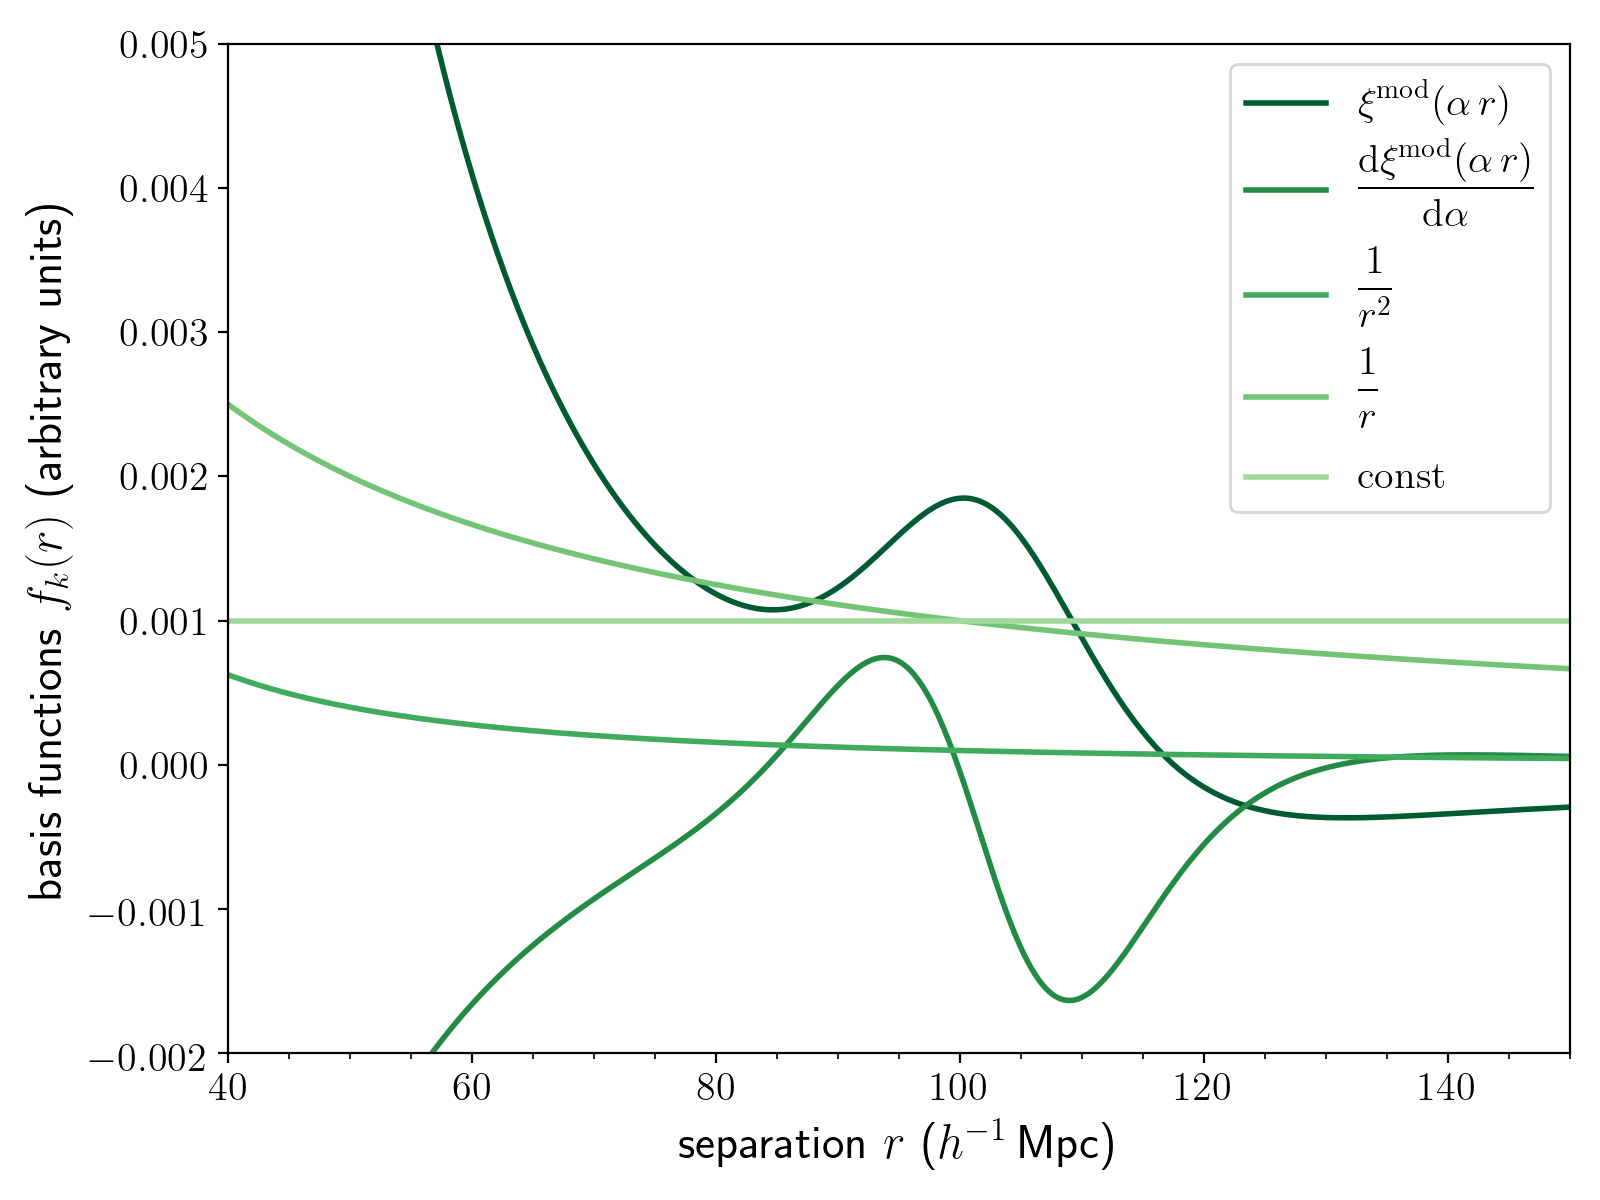
\includegraphics[width=0.8\textwidth]{bao_bases}
    \caption{The set of basis functions used to fit for the BAO scale using our estimator. The $B^2$ term (green) is the fiducial model used to determine the scale dilation parameter $\alpha$. The $C$ term is the derivative of this model with respect to $\alpha$, allowing for the estimation of this parameter. The $a_1$, $a_2$, and $a_3$ terms are nuisance parameters to fit the broadband shape. \KSF{Make colorblind friendly! and diff linewidths maybe}}
\end{figure}

We demonstrate this method using the same set of lognormal mocks as in $\S$\ref{sec:spline}.
We construct a recovery test following that in \cite{Hinton2019}.
We assume the fiducial cosmological model used in \cite{Beutler2017}: $\Omega_{\text{m}} = 0.31$, $h = 0.676$, $\Omega_{\text{b}} = 0.04814$, $n_s = 0.97$. 
As we know the cosmology used for our mock catalogs, we can compute the true value of the scale dilation parameter, $\alpha_{\text{true}}=0.9574$ (a fairly extreme value but useful for testing purposes).
With this fiducial model, we can construct the basis functions for our estimator; these are shown (with $\alpha=1$ and the free parameters set to arbitrary values) in Figure~\ref{fig:bao_bases}.

We perform an iterative procedure to estimate $\alpha$.
After the first estimation with the $\alpha=1$, model, we use the value of $C$ to compute the recovered $\alpha$, as described above.
We then take that value as the new $\alpha$, and re-run the estimator.
(In practice, this often jumps over the true value, so we tune the choice of the next $\alpha$ with a parameter $\eta$, as $\alpha_{\text{recovered}} = \alpha + \eta C d\alpha$, where $\eta$ is typically 0.1-0.5.)
We stop when the percent change between $\alpha$ and $\alpha_{\text{recovered}}$ is less than 0.1\%; it typically takes fewer than 10 iterations to converge. \KSF{update this with true values}
We apply this procedure to each of the 100 mocks; the resulting estimate for the correlation function is shown in Figure~\ref{fig:bao}.
The mean BAO estimate is shown in orange, and the mean tophat estimate is in blue; the truth is in black.
Our estimator clearly better represents the shape of the known \cf.
The mean value of the final recovered scale dilation parameter is $\alpha=0.9572 \pm 0.0315$, very close to the true value $\alpha_{\text{true}}=0.9574$.

\label{fig:bao}
\begin{figure}[th]
\centering
    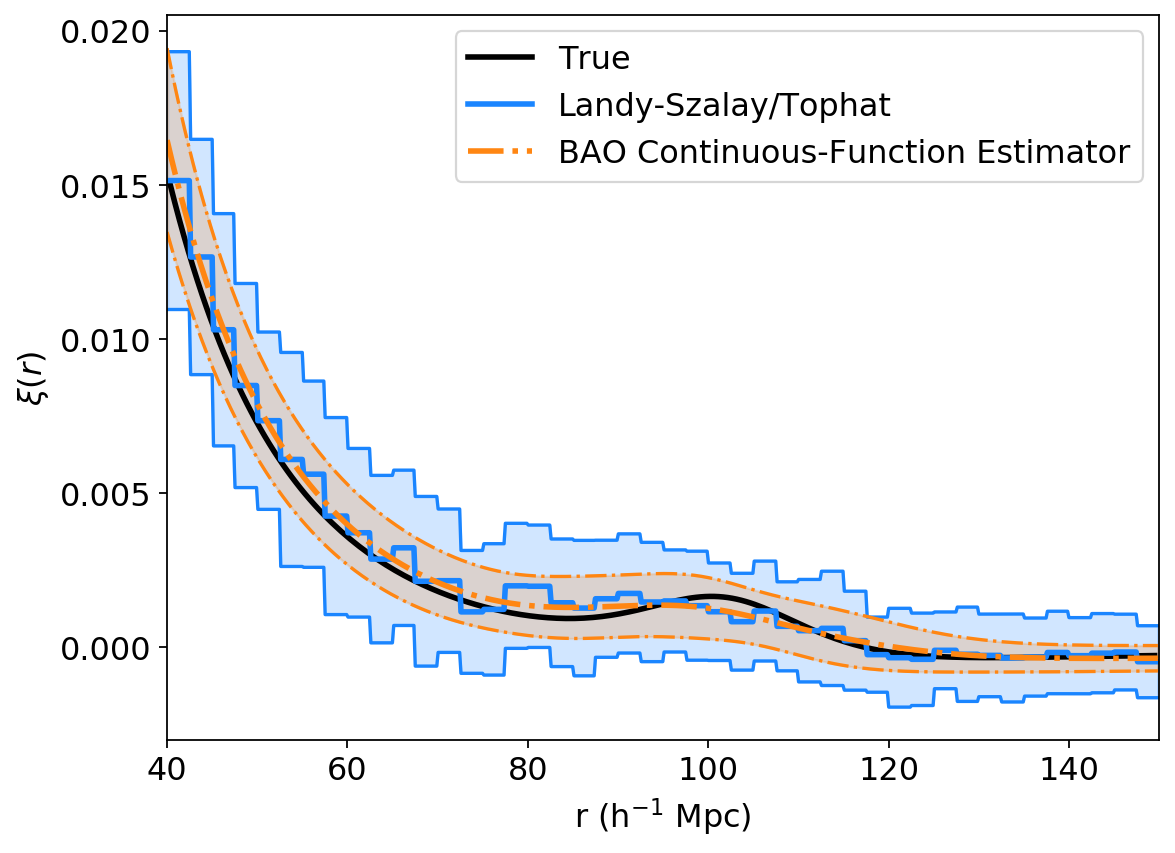
\includegraphics[width=0.8\textwidth]{bao}
    \caption{Estimation of the correlation function using our estimator with basis functions based on the BAO fitting function (orange dot-dashed). The line is the mean of the final estimate from the iteration procedure for 100 mocks, and the shaded region is the $1\sigma$ variation. We also show the standard Landy-Szalay estimator, displayed as a tophat function (blue), as well as the true input correlation function (black). \KSF{This is for the 1e-4 box, need to run bigger box.} \KSF{Should this and the basis set figure be a single figure with two panels?} \KSF{Should i have a figure showing the sum of the basis functions and how that gets you the final cf?}}
\end{figure}

We note that these basis functions are significantly different than the tophat or B-spline bases previously explored, mainly because they are not localized.
This means that data at all scales could contribute to all basis functions.
It is then critical to ensure that the final parameter estimate does not rely on the range of scales chosen.
We have confirmed that in this application, the result is robust to the chosen range as long as the scales cover the range $40<r<200$ \hmpc, the typical range used in BAO analyses. \KSF{Actually have to check this and update numbers!}


\section{Discussion} \label{sec:discuss}

\subsection{Relationship to Other Existing Estimators}

\Est has properties similar to existing estimators, including kernel density estimators and the marked correlation function.
With the proper choice of basis functions, \est can indeed produce both of these estimators; it is more general than either of them.

Kernel density estimation (KDE) is a class of methods for estimating a probability density function from a set of data.
KDE methods essentially smooth the data with a given kernel, often a Gaussian.
\KSF{should i cite the original KDE papers from the 50s and 60s? or not necessary bc not the focus?}
This is useful when we want to reconstruct a distribution without making many assumptions about the data, as is required in parametric methods.
KDEs have found use in many areas of astrophyics, for example to measure the 21cm power spectrum with reduced foreground contamination \citep{Trott2019}, and to estimate luminosity functions with superior performance compared to binned methods \citep{Yuan2020}.
\KSF{there are others, should i list more citations? without describing?}
\cite{Hatfield2016} uses a KDE approach to estimate the angular correlation function, in order to address the issues of information loss and arbitrary bin choice inherent to binning; they optimize for the kernel choice, and find a correlation function consistant with that of the binned method.
\KSF{I couldnt find any other papers that use KDEs on correlation functions, but i found this one by chance. more to say here? the paper doesn't draw strong conclusions from this.}

Specifically, kernel density estimators take the contribution of each data point to be a kernel function centered on that value, and sum these to determine the full distribution.
In contrast, \est projects each data point onto fixed basis functions, which are distinct from the typical understanding of kernels.
As such, our estimator is not smearing out the data, as KDEs do; it is using the data to directly infer the contribution of each basis function.
That said, the formulation of \est is general enough that it can perform a kernel density estimate of the correlation function, by choosing $f(r)$ to be a kernel centered on $r$.
However, our uses here of the estimator are fundamentally different from KDE methods, as they use use fixed basis functions that can take advantage of the science use case and preserve maximal information from the data.
\KSF{this last sentence is a bit repetitive / are there more differences im missing?}

\KSF{Paragraph on marked cf}

\label{ref:beyondls}
\subsection{Beyond the Landy-Szalay Estimator}

While we have formulated our estimator as a generalization of \LS, as it is the standard used in \cf analyses and has optimal properties under certain conditions, we can also reformulate it for other estimators.
The formulation currently requires a normalization term (i.e. denominator) of the $RR$ counts, as we replace this with our $QQ$ term.
This is the case for the \cite{PeeblesHauser1974} estimator and the \cite{Hewett1982} estimator:
\begin{eqnarray}
    \xi_{PH}(r) &=& \frac{DD - RR}{RR} \\
    \xi_{Hew}(r) &=& \frac{DD - DR}{RR}.
\end{eqnarray}
\KSF{dropped $k$ and $(r)$ notation here, do i need?}
We could also generalize estimators which have a $DR$ term as the denominator, such as the \cite{DavisPeebles1983} estimator,
\begin{equation}
    \xi_{DP}(r) = \frac{DD - DR}{DR}
\end{equation}
by defining
\begin{equation}
    DQ = \frac{2}{N_D N_R} \sum_{n m} f(T_n, T_m) \cdot f\T(T_n, T_m).
\end{equation}
This could be extended to almost any linear combination of pair counts.
The estimator of \cite{VargasMagana2013} selects the optimal combination of pair counts; our estimators could be combined to create an even more generalized estimator.
\KSF{some of the terms in V-M include DD in the denom - need to mention this?}

\KSF{Mention other work with Barnett about LS estimator?}

\KSF{not sure where this next paragraph belongs}
We also note that the \est can be easily generalized to cross-correlations between two datasets.
In this case, we consider datasets $D_1$ and $D_2$, and associated random catalogs $R_1$ and $R_2$. 
We then have two different data-random terms, crossing each dataset with the opposite random catalog, resulting in a \LS estimator of the form
\KSF{notation is now clunky with double subscripts; could make 1 and 2 superscript? or maybe it's fine with the parens}
\begin{equation}
    \hat{\xi}_k = \frac{(D_1 D_2)_k - (D_1 R_2)_k - (D_2 R_1)_k + (R_1 R_2)_k}{(R_1 R_2)_k}.
\end{equation}
Here, each term is normalized simply by the number of pairs, as
\begin{equation}
    D_1 D_2 \equiv \frac{1}{N_{D1} N_{D2}} \sum_{n n'} f(T_n, T_{n'})
\end{equation}
and similarly for the other terms.
This cross-correlation formulation can be extended to other estimators beyond \LS in a straightforward way.

\subsection{Computational Performance}

The computational scaling is by definition the same as traditional estimators, because pair-finding remains the limiting factor.
\Est has the additional need for evaluating the function $f$ for each pair of galaxies.
For simple basis functions like splines, this will only marginally decrease performance.
For more complicated functions such as evaluating a cosmological model, \est may incur extra computational expense.
Basis functions can also be input on a grid and then interpolated; the performance is then the same for all functions, but the interpolation for each function for each pair does somewhat decrease the performance.

\KSF{Is there a need to say much more? If not, maybe doesn't deserve its own section - could this go in the implementation section? Or maybe tacked onto another small section if we have one that makes sense}

\subsection{Effect on Covariance Matrix Estimation}

We have shown that \est results in \cf estimates that are just as accurate with fewer components.
This is critical when estimating the covariance matrix, which is necessary for parameter inference.
The covariance matrix is difficult to compute theoretically;instead, it is usually estimated by evaluating the \cf on a large number of mock catalogs and computing the covariance between the bins (e.g. \citealt{Reid2010}; \citealt{Anderson2014}).
The unbiased estimator for the sample covariance matrix is (e.g. \citealt{Anderson2003})
\begin{equation}
\hat{C}^{ML}_{ij} = \frac{1}{N_{mocks}-1} \sum_{k=1}^{N_{mocks}} \bigg( x^k_i - \bar{x}_i \bigg) \bigg( x^k_j - \bar{x}_j \bigg),
\end{equation}
where $k$ denotes the index of the mock, $i$ and $j$ denote the index of the bin or component, $x$ denotes the estimate in that bin for that mock, and $\bar{x}$ denotes the mean value of the estimate in that bin across the mocks.
To get an unbiased estimate of the inverse covariance matrix, we require a correction factor, as the inverse of an unbiased estimator is not necessarily unbiased.
The unbiased estimator for the sample inverse covariance matrix can be shown to be \citep{Hartlap2007}
\begin{equation}
\hat{C}\inv = \frac{N_{mocks}-N_{bins}-2}{N_{mocks}-1} \bigg( \hat{C}^{ML}\bigg) \inv.
\end{equation}

%This prefactor correction results in the  propagates to the variance in 
The variance in the elements of this estimator then have a dependence on $N_{mocks}$ and $N_{bins}$.
This propagates to the derived cosmological parameters, resulting in an overestimation of the error bars (\citealt{Hartlap2007}; \citealt{Dodelson2013} \citealt{Percival2014}; \citealt{TaylorJoachimi2014}).
Assuming that $N_{mocks} >> N_{bins}$ (and both much larger than the number of parameters to be estimated), and that the measurements are Gaussian distribued, the error bars are inflated by a factor of $(1 + N_{bins}/N_{mocks})$ (i.e., the true constraints are tighter than the derived ones).
This factor becomes critical at the precision of cosmological parameter estimation \citep{Percival2014}.

Typically, this is dealt with by generating a very large number of mocks.
For the Baryon Oscillation Spectroscopic Survey (BOSS, \citealt{Dawson2013}), $\sim$600 mocks were needed and the analysis used 41 bins \citep{Sanchez2012}.
Future surveys will have more costly requirements on mock catalogs, with larger simulations necessary to cover the larger survey volumes.

An alternative to increasing $N_{mocks}$ is decreasing $N_{bins}$ to achieve the same error on precision.
In the standard method, this is shown to \emph{increase} the statistical error, albeit only slightly \cite{Percival2014}.
A substantial increase in bin width would prevent capturing information in finer clustering features; even the relatively broad BAO peak requires a bin size on the order of its width of $\sim$10\hmpc.
In fact, in the standard method more bins would typically be desireable, but the number is limited by the available number of mocks for covariance matrix computation.

With our estimator, we have shown that we can reduce the variance by using fewer components, without sacrificing accuracy.
This means that we can safely reduce $N_{bins}$, or in our replacement of bins with continuous functions, the number of basis functions $K$.
The covariance matrix will be the covariance between these basis functions. \KSF{worth noting that the structure of this covmat will be significantly different, esp if non-orthogonal?}
To then achieve the same precision on the error on the cosmological parameters, a lower value of $N_{mocks}$ becomes possible.
This will significantly reduce requirements on mocks, which will be particularly important for upcoming large surveys. 

\KSF{I think the result of discussions was that there wasn't a good way of showing this without propagating all the way to cosmological parameters. Would love a figure showing lower covariance errors but not sure how without full propagation}

\subsection{Further Applications}

The formulation of \est opens up many possibilities for extracting information from the correlation function.
The most straightforward applications are standard basis functions or linearizeable astrophysical models, as we have shown here.
Other applications for the direct estimation of cosmological parameters could include the growth rate of cosmic structure $f$ \citep{Satpathy2016, Reid2018} and primordial non-Gaussianity in the local density field $f^{local}_{NL}$ \citep{Karagiannis2014}.
\KSF{mention idea of doing full cosmo model analysis by taking derivs wrt cosmological params? cool but less connected to citeable papers perhaps}

We can take our estimator a step further by choosing basis functions that depend not only on the separation between tracer pairs, but also on the properties of the tracers themselves.
One such application is the redshift dependence of the Alcock-Paczynski effect \cite{AlcockPaczynski1979}, which can be used to constrain the matter density $\Omega_m$ and the dark energy equation of state parameter $w$ \citep{Li2016}.
The basis functions $f$ in this case would take the form
\begin{equation}
    f_k(T_n, T_m) = f_k(r_{nm}, z_n, z_m),
\end{equation}
where $z$ is the redshift of tracer $n$ or $m$.
Another potential use case is the luminosity and color dependence of galaxy clustering, which can be used to understand the relationship between galaxy formation and the LSS \citep{Zehavi2011}.
This could be extended to other galaxy properties.

The estimator gives us the opportunity to investigate more subtle or exotic signals which are anomalous with respect to our conventional models.
Anomalies could appear as inhomogeneities or anisotropies in the data.
For example, cosmological parameters could vary across the sky, which has previously investigated in patches across the Cosmic Microwave Background \citep{MukherjeeWandelt2018}.
Another possibility is anisotropy in the cosmic acceleration, which could leave signatures in measurements made using various phenomena including baryon acoustic oscillations \citep{Faltenbacher2012} and Type Ia supernovae \citep{Colin2019}.
With our estimator, we could introduce a dependence on location or direction into our basis functions, and constrain the potential deviation from homogeneity or isotropy.
While these effects would be highly degenerate with systematics, our estimator combined with robust systematics mitigation allows us to investigate the possibility of new physics.

Finally, our estimator can be directly related to a power spectrum analysis.
We could use a Fourier basis as our set of continuous functions.
This would allow us to directly project the data onto Fourier modes.
This represents a step towards unifying the correlation function and the power spectrum. \KSF{there's more to say here but I'm not sure what}


\section{Summary}

\KSF{TODO: write short summary}

\acknowledgements
KSF was supported by the NASA FINESST grant [grant number] during the completion of this work.
The authors thank Jeremy Tinker and Michael Blanton for helpful discussions, Roman Scoccimarro for insightful conversation, and the members of the Flatiron Astronomical Data Group for useful feedback.
KSF would like to acknowledge significant code feedback and support from Manodeep Sinha, as well as Lehman Garrison.
KSF thanks Drew Jamieson, Chris Lovell for helpful discussion...
All of the code used in this paper is available open-source at \texttt{github.com/kstoreyf/Corrfunc} and \texttt{github.com/kstoreyf/continuous-estimator}. 

\appendix
\section{Affine Invariance}\label{sec:affine}

The estimator is invariant under an affine transformation. We represent this by a transformation matrix M, such that 
\begin{equation}
f' \leftarrow Mf
\end{equation}
Then in the primed basis, the pair counts become
\begin{eqnarray}\displaystyle
DD' &=& \sum_{n n'} M f_{n n'} = M\,DD
\\
DR' &=& \sum_{n m} M f_{n m} = M\,DR
\\
RR' &=& \sum_{m m'} M f_{m m'} = M\,RR
\end{eqnarray}
where $f_{n n'} = f_k(T_n, T_{n'})$.
We have factored $M$ out of the summation. For the $QQ$ tensor we have
\begin{eqnarray}\displaystyle
QQ' &=& \sum_{m m'} (Mf_{m m'}) \cdot (Mf_{m m'})\T \\
&=& M\Bigg[ \sum_{m m'} f_{m m'} \cdot f_{m m'}\T \Bigg]M\T \\
&=& M QQ M\T
\end{eqnarray}
Then the amplitudes in the primed basis become
\begin{eqnarray}\displaystyle
a' &=& [M QQ M\T]\inv \cdot [MDD - 2\,MDR + MRR] \\
&=& (M\T)\inv QQ\inv \cdot [DD - 2\,DR + RR] \\
&=& (M\T)\inv a
\end{eqnarray}
and the estimator in the primed basis is 
\begin{eqnarray}\displaystyle
\xi' &=& [(M\T)\inv a]\T \cdot (Mf) \\
&=& a\T[(M\inv)\T]\T \cdot (Mf) \\
&=& a\T M\inv \cdot Mf \\
&=& a\T \cdot f = \xi.
\end{eqnarray}
Thus after an affine transformation of the basis function, the resulting estimator is equivalent to the estimator in the original basis.

We note that this requires $M$ be invertible.
% not sure if i understand what i wrote here
However, any two equivalent bases must be related by the inverse of a transformation matrix, so this requirement is already satisfied.


\section{Computing RR and QQ Analytically}\label{sec:analytic}

The autocorrelation of the random catalog is meant to approximate the window function. 
When we have a periodic cube, we can compute this $RR$ term analytically.
Here we derive this, and then derive the equivalent for our continuous-basis $RR$ and $QQ$ terms.

We consider an annulus around a single galaxy. 
This annulus has a volume $V_{ann}$.
Taking the box to have average number density $\bar{n}$, the number of galaxies expected in the annulus is $N_{ann} = A \bar{n}$, and thus this galaxy is part of $N_{ann}$ pairs.   
We do this for each of the $N_D-1$ other galaxies, and find a total of $(N_D-1) N_{annulus} = \frac{1}{2} (N_D-1) V_{ann} \bar{n}$ pairs, where the factor of $\frac{1}{2}$ accounts for the fact that this double-counts pairs.
For a cube, $\bar{n} = \frac{N_D}{L^3}$, so we finally count $\frac{1}{2} \frac{N_D}{L^3} (N-1) V_{ann}$ pairs.

For hard-edged radial bins, we can compute $A$ simply as the difference between spherical volumes. 
We can also represent this as an integral:
\begin{equation} \label{eq:vol_tophat}
V_{ann} = \int_{b_1}^{b_2} dV = 4\pi \int_{b_1}^{b_2} r^2 dr
\end{equation} 
We can generalize this to any basis function $f(r)$ that is a function of $r$:
\begin{equation}
V_{ann} = 4\pi  \int_{b_1}^{b_2} f^2(r) r^2 dr
\end{equation}
which we can see reduces to Equation \ref{eq:vol_tophat} when $f(r)$ is the tophat function (returning 1 or 0 depending on whether $r$ is between $b_1$ and $b_2$).

This gives us our full generalized analytic $RR$ term, which has elements
\begin{equation}
RR_{i,\text{ana}} = \frac{1}{2} \frac{N_D}{L^3} (N_D-1)  4\pi  \int_{0}^{r_\mathrm{max}} f_i(r) r^2 dr
\end{equation}
where $i$ is the index of the basis function vector.
Based on the definition of $QQ$ in Equation \ref{eq:qq_proj} as the outer product of the basis function vector and its transpose, we can see that the elements analytic $QQ$ term are:
\begin{equation}
QQ_{ij,\text{ana}} = \frac{1}{2} \frac{N_D}{L^3} (N_D-1)  4\pi  \int_{0}^{r_\mathrm{max}} f_i(r) f_j(r) r^2 dr
\end{equation}
This could be further generalized to account for basis functions that take other properties as input.

When considering a periodic box, the naive estimator is no longer biased, so we can also avoid computing the $DR$ term and calculate the amplitudes as 
\begin{equation}
a_{\mathrm{ana}} = QQ_\mathrm{ana} \inv \cdot DD.
\end{equation}
Looking back, it might have seemed strange that we use $N_D$ in calculating the analytical $RR$ term, but we now see that this normalization prefactor cancels out with that of the $DD$ term.
Finally, we can compute the correlation function as before in Equation \ref{eq:xi_proj}.

\section{Iterative Procedure for Estimating the BAO Basis Functions}\label{sec:baoiter}

The \est can be used to measure the baryon acoustic oscillation (BAO) scale by choosing the basis functions to be BAO fitting functions, as described in \ref{sec:app}. \KSF{check/update reference}
For this application, we need to choose a fiducial cosmology for our bases, which will be offset from the true cosmology.
This offset can be encoded by a scale dilation parameter $\alpha$, which contains the information about the BAO scale. \KSF{reference proper eqn}
As our fitting function requires a numerical derivative to estimate $\alpha$, we require an iterative procedure to converge to the best-fit value. \KSF{this doesn't quite capture why iterative; clarify}

We start with assuming that we have chosen our fiducial model to match our true cosmology (we in all likelihood have not, but it's not a bad initial guess).
This gives us an initial $\alpha_\mathrm{model} = 1$. 
We also choose a value for $d\alpha$, how much we will change our model by to compute the numerical derivative; we take it to be $d\alpha=0.01\alpha_\mathrm{model}$. 

We then apply \est to perform the measurement, and obtain the amplitude for the derivative term in our model, $C$, as in Equation \ref{eq:baoiter_fit}. 
This gives us the naive best-fit $\alpha$ from this initial model,
\begin{equation}
    \alpha_\mathrm{result} = \alpha_\mathrm{model} + \eta C d\alpha
\end{equation}
where $\eta$ is a damping parameter between $0$ and $1$.
If $\eta$ is too large, this can result in ``jumps'' to the next $\alpha$ value that are too large, and leap over the best value; this can lead to a back-and-forth cycle in which the result hops between two values and never converges.
In our application, we choose $\eta=0.2$ for the first 50 iterations, and then reduce it for subsequent iterations \KSF{describe exactly how!}.

We choose a convergence criterion to be when the fractional change in $\alpha_\mathrm{result}$ between subsequent iterations falls below a threshold, $c_\mathrm{thresh}$ \KSF{name for this variable?}.
As we are using the previous iteration's $\alpha_\mathrm{result}$ as the $\alpha_\mathrm{model}$ for the current iteration, we have
\begin{equation}
    c_\mathrm{thresh} = \frac{\alpha_\mathrm{model} - \alpha_\mathrm{result}}{\alpha_\mathrm{model}}.
\end{equation}
We choose a threshold of $c_\mathrm{thresh} = 0.0001$.

\KSF{does this next bit make sense?}
However, with this definition, the convergence will have a dependence on the choice of $\eta$.
To avoid this, we could choose the $\alpha_\mathrm{result}$ for the convergence criterion to be the result if $\eta=1$, $\alpha_{\mathrm{result},\eta=1}$.
Then the criterion is
\begin{equation}
    c_\mathrm{thresh} = \frac{\alpha_\mathrm{model} - \alpha_{\mathrm{result},\eta=1}}{\alpha_\mathrm{model}}.
\end{equation}
If the criterion is not met, we use the damped $\alpha_\mathrm{result}$ as the $\alpha_\mathrm{model}$ for the next iteration.
If the criterion is met, we take $\alpha_{\mathrm{result},\eta=1}$ as our final result. 
\KSF{or should this be just $\alpha_\mathrm{result}$, not $\eta=1$??}

%need style file error
%\bibliographystyle{apj} 
%\bibliography{paper}
% To copy from mendeley locally: in paper dir, [cp ~/code/bibtex/LSS-est_paper.bib .]
\bibliography{LSS-est_paper}

\end{document}














